\begin{savequote}[45mm]
\ascii{Any fool can write code that a computer can understand. Good programmers write code that humans can understand.}
\qauthor{\ascii{- Martin Flower}}
\end{savequote}

\chapter{编程环境} 
\label{ch:prog-env}

\begin{content}

为了实现\tf{}的快速入门,本章将介绍\tf{}的编程环境,包括代码结构,工程构建,环境验证,以便对\tf{}有一个基本的感性认识。

\end{content}

\section{代码结构}

\begin{content}

\subsection{克隆源码}

首先,从\ascii{Github}上克隆\tf{}的源代码。


\begin{leftbar}
\begin{python}
$ git clone git@github.com:tensorflow/tensorflow.git
\end{python}
\end{leftbar}

然后,切换到最新的稳定分支上。例如,\code{r1.2}分支。

\begin{leftbar}
\begin{python}
$ cd tensorflow
$ git checkout r1.2
\end{python}
\end{leftbar}

\subsection{源码结构}

可以运行如下命令,打印出\tf{}源码的组织结构。

\begin{leftbar}
\begin{python}[]
$ tree -d -L 1 ./tensorflow
\end{python}
\end{leftbar}

其中,本书将重点关注\code{core, python, c}组件,部分涉及\code{cc, stream\_executor}组件。

\begin{leftbar}
\begin{c++}[caption={TensorFlow源码结构}]
./tensorflow
├── c
├── cc
├── compiler
├── contrib
├── core
├── docs_src
├── examples
├── g3doc
├── go
├── java
├── python
├── stream_executor
├── tools
└── user_ops
\end{c++}
\end{leftbar}

\subsection{内核}

内核的源码物理组织如下所示。主要包括平台,实用函数库,\ascii{Protobuf}定义,本地和分布式运行时,框架,图结构,及其\ascii{OP}定义与\ascii{Kernel}实现等组成,这也是本书重点剖析的对象。

\begin{leftbar}
\begin{c++}[caption={内核源码结构}]
./tensorflow/core
├── common_runtime
├── debug
├── distributed_runtime
├── example
├── framework
├── graph
├── grappler
├── kernels
├── lib
├── ops
├── platform
├── profiler
├── protobuf
├── public
├── user_ops
└── util
\end{c++}
\end{leftbar}

\subsection{Python接口}

Python编程接口的源码物理组织如下所示,它定义和实现了程序员的编程接口,这也是本书重点剖析的对象。

\begin{leftbar}
\begin{c++}[caption={Python源码结构}]
./tensorflow/python
├── client
├── debug
├── estimator
├── feature_column
├── framework
├── grappler
├── kernel_tests
├── layers
├── lib
├── ops
├── platform
├── profiler
├── saved_model
├── summary
├── tools
├── training
├── user_ops
└── util
\end{c++}
\end{leftbar}

\subsection{StreamExecutor}

\ascii{StreamExecutor}是\ascii{Google}另一个组件库,但它也是\ascii{TensorFlow}计算的核心引擎,本书将大体介绍其系统架构与工作原理。

\begin{leftbar}
\begin{c++}[caption={StreamExecutor源码结构}]
./tensorflow/stream_executor
├── cuda
├── host
├── lib
└── platform
\end{c++}
\end{leftbar}

\end{content}

\section{工程构建}

\begin{content}

因篇幅受限,本文仅以\ascii{Mac OS}为例,讲述\tf{}的源码编译、安装、及其验证过程。其他操作系统,及其\ascii{CUDA}环境安装,请查阅\tf{}官方文档。

\subsection{环境准备}

在构建\ascii{TensorFlow}前,需要事先准备构建环境。\ascii{TensorFlow}的前端是一个支持多语言的编程接口,后端是一个使用\ascii{C++}实现的执行系统。

因此,编译\ascii{TensorFlow}源代码之前,需要事先安装前端系统所使用编程语言的编译器、解释器、及其运行时环境。例如,使用\ascii{Python}的前端编程接口,需要事先安装\ascii{Python2},或者\ascii{Python3}。下文以\ascii{Python2}为例,讲述环境准备过程;如果使用\ascii{Python3},请查阅相关文档。

其次,也需要事先安装\ascii{GCC, Clang}等\ascii{C++}的编译器,用于编译后端系统实现。本文将不再冗述这两个方面的环境安装过程。

另外,\ascii{TensorFlow}使用\ascii{Bazel}的构建工具。因此,需要事先安装\ascii{Bazel}。不幸的是,因为\ascii{Bazel}依赖于\ascii{JDK},因此在安装\ascii{Bazel}之需要前先安装\ascii{JDK}。

\subsubsection{安装JDK}

可以从\ascii{Oracle}官网上下载至少\ascii{1.8}及以上版本的\ascii{JDK}版本,然后安装在系统中。

\begin{leftbar}
\begin{python}
$ sudo mkdir -p /usr/lib/jvm
$ sudo tar zxvf jdk-8u51-linux-x64.tar.gz -C /usr/lib/jvm
$ sudo ln -s /usr/java/jdk1.8.0_51 /usr/java/default
\end{python}
\end{leftbar}

创建\ascii{Java}相关环境变量,并添加到\code{~/.bashrc}配置文件中。

\begin{leftbar}
\begin{python}
$ echo 'export JAVA_HOME=/usr/java/default' >> ~/.bashrc
$ echo 'export PATH="$JAVA_HOME/bin:$PATH"' >> ~/.bashrc
\end{python}
\end{leftbar}

生效环境变量。

\begin{leftbar}
\begin{python}
$ source ~/.bashrc
\end{python}
\end{leftbar}

\subsubsection{安装Bazel}

在\ascii{Mac OS}上,可以使用\ascii{brew}安装\ascii{Bazel}。

\begin{leftbar}
\begin{python}
$ brew install bazel
\end{python}
\end{leftbar}

如果系统未安装\ascii{brew},可以执行如下命令先安装\ascii{brew}。当然,需要事先安装\ascii{Ruby}解释器,在此不再冗述。

\begin{leftbar}
\begin{python}
$ /usr/bin/ruby -e "$(curl -fsSL https://raw.githubusercontent.com/Homebrew/install/master/install)"
\end{python}
\end{leftbar}

\subsubsection{安装Swig}

\ascii{TensorFlow}使用\ascii{Swig}构建多语言编程的环境,因此需要事先安装\ascii{Swig}工具包。

\begin{leftbar}
\begin{python}
$ brew install swig
\end{python}
\end{leftbar}

\subsubsection{安装Python依赖包}

使用\ascii{pip}安装\ascii{TensorFlow}所依赖的\ascii{Python}包。

\begin{leftbar}
\begin{python}
$ sudo pip install six numpy wheel
\end{python}
\end{leftbar}

如果系统未安装\ascii{pip},则可以使用\ascii{brew}先安装\ascii{pip}:

\begin{leftbar}
\begin{python}
$ brew install pip
\end{python}
\end{leftbar}

\subsection{配置}

编译环境准备就绪之后,便可以执行\code{./configure}配置\ascii{TensorFlow}的编译环境了。特殊地,当系统不支持\ascii{GPU},则可以不需要配置和安装\ascii{CUDA},及其\ascii{cuDNN}。

\begin{leftbar}
\begin{python}
$ ./configure
\end{python}
\end{leftbar}

\subsection{构建}

当配置成功后,使用\ascii{Bazel}启动\ascii{TensorFlow}的编译。特殊地,当需要支持\ascii{GPU}时,添加\code{--config=cuda}编译选项。

\begin{leftbar}
\begin{python}
$ bazel build --config=opt //tensorflow/tools/pip_package:build_pip_package
\end{python}
\end{leftbar}

编译成功后,便可以构建\ascii{TensorFlow}的\ascii{Wheel}包。

\begin{leftbar}
\begin{python}
$ bazel-bin/tensorflow/tools/pip_package/build_pip_package /tmp/tensorflow_pkg
\end{python}
\end{leftbar}

\subsection{安装}

当\ascii{Whell}包构建成功后,便可以使用\ascii{pip}安装\ascii{TensorFlow}了。

\begin{leftbar}
\begin{python}
$ sudo pip install /tmp/tensorflow_pkg/tensorflow-1.2.0-py2-none-any.whl
\end{python}
\end{leftbar}

\subsection{验证}

启动\ascii{Python}解释器,验证\ascii{TensorFlow}安装是否成功。

\begin{leftbar}
\begin{python}
$ python
>>> import tensorflow as tf
>>> hello = tf.constant('Hello, TensorFlow!')
>>> sess = tf.Session()
>>> print(sess.run(hello))
Hello, TensorFlow!
\end{python}
\end{leftbar}

\end{content}

\section{技术栈}

\begin{content}

通过构建\ascii{TensorFlow}源码,应该对\ascii{TensorFlow}所依赖的构建工具、组件库、及其第三方工具包有了初步的感性认识。

按照\ascii{TensorFlow}的系统软件层次,通过一张表格罗列\ascii{TensorFlow}所使用的技术栈,以便更清晰地了解\ascii{TensorFlow}的生态系统。

\begin{figure}[!htbp]
\centering
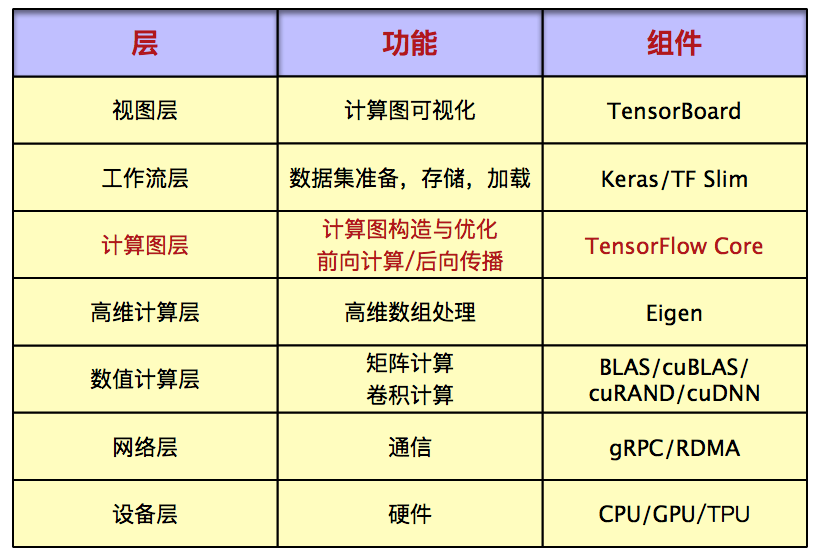
\includegraphics[width=0.7\textwidth]{figures/tf-stack.png}
\caption{TensorFlow技术栈}}
 \label{fig:tf-stack}
\end{figure}

\end{content}
